\chapter{数论}

\index{数论}

\key{数论}是数学的一个分支，
研究整数。
数论是一个令人着迷的领域，
因为许多涉及整数的问题
即使乍一看很简单，
也非常难以解决。

作为一个例子，考虑以下方程：
\[x^3 + y^3 + z^3 = 33\]
很容易找到三个实数 $x$、$y$ 和 $z$
满足该方程。
例如，我们可以选择
\[
\begin{array}{lcl}
x = 3, \\
y = \sqrt[3]{3}, \\
z = \sqrt[3]{3}.\\
\end{array}
\]
然而，是否存在三个\emph{整数} $x$、$y$ 和 $z$
满足该方程，
是数论中的一个未解决的问题 \cite{bec07}。

在本章中，我们将重点讨论数论中的基本概念
和算法。
在本章中，除非另有说明，
我们假设所有数都是整数。

\section{素数与因子}

\index{整除性}
\index{因子}
\index{因数}

如果 $a$ 整除 $b$，
则称 $a$ 为 $b$ 的\key{因子}或\key{因数}。
如果 $a$ 是 $b$ 的因子，
我们记为 $a \mid b$，否则记为 $a \nmid b$。
例如，24 的因子有
1、2、3、4、6、8、12 和 24。

\index{素数}
\index{素数分解}

如果一个数 $n>1$ 的正因子只有 1 和 $n$，
则称 $n$ 为\key{素数}。
例如，7、19 和 41 是素数，
但 35 不是素数，因为 $5 \cdot 7 = 35$。
对于每个数 $n>1$，都存在唯一的
\key{素数分解}
\[ n = p_1^{\alpha_1} p_2^{\alpha_2} \cdots p_k^{\alpha_k},\]
其中 $p_1,p_2,\ldots,p_k$ 是互不相同的素数，
$\alpha_1,\alpha_2,\ldots,\alpha_k$ 是正整数。
例如，84 的素数分解为
\[84 = 2^2 \cdot 3^1 \cdot 7^1.\]

数 $n$ 的\key{因子个数}为
\[\tau(n)=\prod_{i=1}^k (\alpha_i+1),\]
因为对于每个素数 $p_i$，
有 $\alpha_i+1$ 种方式选择
它在因子中出现的次数。
例如，84 的因子个数为
$\tau(84)=3 \cdot 2 \cdot 2 = 12$。
这些因子是
1、2、3、4、6、7、12、14、21、28、42 和 84。

$n$ 的\key{因子之和}为
\[\sigma(n)=\prod_{i=1}^k (1+p_i+\ldots+p_i^{\alpha_i}) = \prod_{i=1}^k \frac{p_i^{a_i+1}-1}{p_i-1},\]
其中后一个公式基于等比数列求和公式。
例如，84 的因子之和为
\[\sigma(84)=\frac{2^3-1}{2-1} \cdot \frac{3^2-1}{3-1} \cdot \frac{7^2-1}{7-1} = 7 \cdot 4 \cdot 8 = 224.\]

$n$ 的\key{因子之积}为
\[\mu(n)=n^{\tau(n)/2},\]
因为我们可以从因子中组成 $\tau(n)/2$ 对，
每对的乘积为 $n$。
例如，84 的因子
组成的对为
$1 \cdot 84$、$2 \cdot 42$、$3 \cdot 28$ 等，
因子之积为 $\mu(84)=84^6=351298031616$。

\index{完全数}

如果一个数 $n$ 满足 $n=\sigma(n)-n$，
即 $n$ 等于 $1$ 到 $n-1$ 之间所有因子之和，
则称 $n$ 为\key{完全数}。
例如，28 是一个完全数，
因为 $28=1+2+4+7+14$。

\subsubsection{素数的个数}

很容易证明素数的个数是无限的。
如果素数的个数是有限的，
我们可以构造一个集合 $P=\{p_1,p_2,\ldots,p_n\}$
包含所有素数。
例如，$p_1=2$，$p_2=3$，$p_3=5$，等等。
然而，利用 $P$，我们可以构成一个新素数
\[p_1 p_2 \cdots p_n+1\]
它比 $P$ 中的所有元素都大。
这是一个矛盾，因此素数的个数
必须是无限的。

\subsubsection{素数的密度}

素数的密度指的是素数在数中出现的频率。
设 $\pi(n)$ 表示 $1$ 到 $n$ 之间的素数个数。
例如，$\pi(10)=4$，因为
$1$ 到 $10$ 之间有 4 个素数：2、3、5 和 7。

可以证明
\[\pi(n) \approx \frac{n}{\ln n},\]
这意味着素数是相当频繁的。
例如，$1$ 到 $10^6$ 之间的素数个数为 $\pi(10^6)=78498$，
而 $10^6 / \ln 10^6 \approx 72382$。

\subsubsection{猜想}

关于素数有许多\emph{猜想}。
大多数人认为这些猜想是正确的，
但没有人能够证明它们。
例如，以下是一些著名的猜想：

\begin{itemize}
\index{哥德巴赫猜想}
\item \key{哥德巴赫猜想}：
每个大于 2 的偶数 $n$ 都可以表示为
两个素数之和 $n=a+b$，即 $a$ 和 $b$ 都是素数。
\index{孪生素数}
\item \key{孪生素数猜想}：
存在无穷多个形如
$\{p,p+2\}$ 的素数对，
其中 $p$ 和 $p+2$ 都是素数。
\index{勒让德猜想}
\item \key{勒让德猜想}：
对于任意正整数 $n$，
在 $n^2$ 和 $(n+1)^2$ 之间总存在一个素数。
\end{itemize}

\subsubsection{基本算法}

如果一个数 $n$ 不是素数，
它可以表示为乘积 $a \cdot b$，
其中 $a \le \sqrt n$ 或 $b \le \sqrt n$，
所以它一定有一个因子在 $2$ 和 $\lfloor \sqrt n \rfloor$ 之间。
利用这个观察，我们可以在 $O(\sqrt n)$ 时间内
测试一个数是否为素数，
以及找出一个数的素数分解。

下面的函数 \texttt{prime} 检查
给定的数 $n$ 是否为素数。
该函数尝试用 $2$ 到 $\lfloor \sqrt n \rfloor$ 之间的
所有数除 $n$，
如果其中没有任何一个能整除 $n$，则 $n$ 是素数。

\begin{lstlisting}
bool prime(int n) {
    if (n < 2) return false;
    for (int x = 2; x*x <= n; x++) {
        if (n%x == 0) return false;
    }
    return true;
}
\end{lstlisting}

\noindent
下面的函数 \texttt{factors}
构造一个包含 $n$ 的素数分解的向量。
该函数用其素因子去除 $n$，
并将它们添加到向量中。
当剩余的数 $n$ 在 $2$ 和 $\lfloor \sqrt n \rfloor$ 之间
没有因子时，过程结束。
如果 $n>1$，则它是素数，也是最后一个因子。

\begin{lstlisting}
vector<int> factors(int n) {
    vector<int> f;
    for (int x = 2; x*x <= n; x++) {
        while (n%x == 0) {
            f.push_back(x);
            n /= x;
        }
    }
    if (n > 1) f.push_back(n);
    return f;
}
\end{lstlisting}

注意，每个素因子在向量中出现的次数
与它整除该数的次数相同。
例如，$24=2^3 \cdot 3$，
所以函数的结果是 $[2,2,2,3]$。

\subsubsection{埃拉托色尼筛法}

\index{埃拉托色尼筛法}

\key{埃拉托色尼筛法}
%\footnote{Eratosthenes (c. 276 BC -- c. 194 BC) was a Greek mathematician.}
是一种预处理
算法，它构建一个数组，
利用该数组我们可以高效地检查 $2 \ldots n$ 之间的给定数
是否为素数，如果不是，则找出该数的一个素因子。

算法构建一个数组 $\texttt{sieve}$，
使用位置 $2,3,\ldots,n$。
值 $\texttt{sieve}[k]=0$ 表示
$k$ 是素数，
值 $\texttt{sieve}[k] \neq 0$
表示 $k$ 不是素数，
且其素因子之一是 $\texttt{sieve}[k]$。

算法逐个遍历 $2 \ldots n$ 的数。
每当发现一个新素数 $x$ 时，
算法记录 $x$ 的倍数
（$2x,3x,4x,\ldots$）不是素数，
因为数 $x$ 能整除它们。

例如，如果 $n=20$，数组如下：

\begin{center}
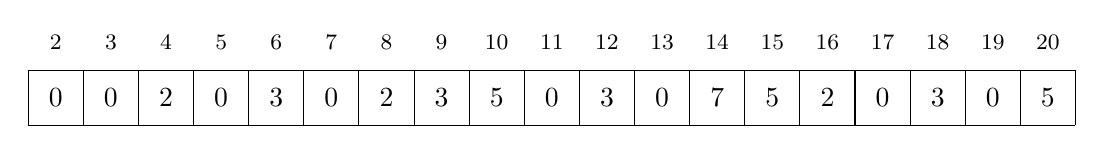
\begin{tikzpicture}[scale=0.7]
\draw (0,0) grid (19,1);

\node at (0.5,0.5) {$0$};
\node at (1.5,0.5) {$0$};
\node at (2.5,0.5) {$2$};
\node at (3.5,0.5) {$0$};
\node at (4.5,0.5) {$3$};
\node at (5.5,0.5) {$0$};
\node at (6.5,0.5) {$2$};
\node at (7.5,0.5) {$3$};
\node at (8.5,0.5) {$5$};
\node at (9.5,0.5) {$0$};
\node at (10.5,0.5) {$3$};
\node at (11.5,0.5) {$0$};
\node at (12.5,0.5) {$7$};
\node at (13.5,0.5) {$5$};
\node at (14.5,0.5) {$2$};
\node at (15.5,0.5) {$0$};
\node at (16.5,0.5) {$3$};
\node at (17.5,0.5) {$0$};
\node at (18.5,0.5) {$5$};

\footnotesize

\node at (0.5,1.5) {$2$};
\node at (1.5,1.5) {$3$};
\node at (2.5,1.5) {$4$};
\node at (3.5,1.5) {$5$};
\node at (4.5,1.5) {$6$};
\node at (5.5,1.5) {$7$};
\node at (6.5,1.5) {$8$};
\node at (7.5,1.5) {$9$};
\node at (8.5,1.5) {$10$};
\node at (9.5,1.5) {$11$};
\node at (10.5,1.5) {$12$};
\node at (11.5,1.5) {$13$};
\node at (12.5,1.5) {$14$};
\node at (13.5,1.5) {$15$};
\node at (14.5,1.5) {$16$};
\node at (15.5,1.5) {$17$};
\node at (16.5,1.5) {$18$};
\node at (17.5,1.5) {$19$};
\node at (18.5,1.5) {$20$};

\end{tikzpicture}
\end{center}

以下代码实现了埃拉托色尼筛法。
代码假设 \texttt{sieve} 的每个元素
初始值为零。

\begin{lstlisting}
for (int x = 2; x <= n; x++) {
    if (sieve[x]) continue;
    for (int u = 2*x; u <= n; u += x) {
        sieve[u] = x;
    }
}
\end{lstlisting}

对于每个 $x$ 的值，算法的内层循环
执行 $n/x$ 次。
因此，算法运行时间的上界是调和级数
\[\sum_{x=2}^n n/x = n/2 + n/3 + n/4 + \cdots + n/n = O(n \log n).\]

\index{调和级数}

事实上，算法更高效，
因为内层循环仅在数 $x$ 为素数时执行。
可以证明算法的运行时间仅为 $O(n \log \log n)$，
这是一个非常接近 $O(n)$ 的复杂度。

\subsubsection{欧几里得算法}

\index{最大公约数}
\index{最小公倍数}
\index{欧几里得算法}

数 $a$ 和 $b$ 的\key{最大公约数}，$\gcd(a,b)$，
是能同时整除 $a$ 和 $b$ 的最大数，
而 $a$ 和 $b$ 的\key{最小公倍数}，
$\textrm{lcm}(a,b)$，
是能同时被 $a$ 和 $b$ 整除的最小数。
例如，
$\gcd(24,36)=12$，
$\textrm{lcm}(24,36)=72$。

最大公约数和最小公倍数
之间的关系如下：
\[\textrm{lcm}(a,b)=\frac{ab}{\textrm{gcd}(a,b)}\]

\key{欧几里得算法}\footnote{欧几里得是一位古希腊数学家，
生活在约公元前 300 年。这可能是历史上第一个已知的算法。}提供了一种高效的方法
来求两个数的最大公约数。
该算法基于以下公式：
\begin{equation*}
    \textrm{gcd}(a,b) = \begin{cases}
               a        & b = 0\\
               \textrm{gcd}(b,a \bmod b) & b \neq 0\\
           \end{cases}
\end{equation*}

例如，
\[\textrm{gcd}(24,36) = \textrm{gcd}(36,24)
= \textrm{gcd}(24,12) = \textrm{gcd}(12,0)=12.\]

该算法可以实现如下：
\begin{lstlisting}
int gcd(int a, int b) {
    if (b == 0) return a;
    return gcd(b, a%b);
}
\end{lstlisting}

可以证明欧几里得算法的
时间复杂度为 $O(\log n)$，其中 $n=\min(a,b)$。
算法的最坏情况是
$a$ 和 $b$ 为连续的斐波那契数。
例如，
\[\textrm{gcd}(13,8)=\textrm{gcd}(8,5)
=\textrm{gcd}(5,3)=\textrm{gcd}(3,2)=\textrm{gcd}(2,1)=\textrm{gcd}(1,0)=1.\]

\subsubsection{欧拉函数}

\index{互素}
\index{欧拉函数}

如果 $\textrm{gcd}(a,b)=1$，
则称数 $a$ 和 $b$ \key{互素}。
\key{欧拉函数} $\varphi(n)$
%\footnote{Euler presented this function in 1763.}
给出 $1$ 到 $n$ 之间与 $n$ 互素的数的个数。
例如，$\varphi(12)=4$，
因为 1、5、7 和 11
与 12 互素。

$\varphi(n)$ 的值可以
从 $n$ 的素数分解中
使用以下公式计算
\[ \varphi(n) = \prod_{i=1}^k p_i^{\alpha_i-1}(p_i-1). \]
例如，$\varphi(12)=2^1 \cdot (2-1) \cdot 3^0 \cdot (3-1)=4$。
注意，如果 $n$ 是素数，则 $\varphi(n)=n-1$。

\section{模运算}

\index{模运算}

在\key{模运算}中，
数的集合是有限的，
只使用 $0,1,2,\ldots,m-1$，
其中 $m$ 是一个常数。
每个数 $x$ 由数 $x \bmod m$ 表示：
即 $x$ 除以 $m$ 的余数。
例如，如果 $m=17$，则 $75$
由 $75 \bmod 17 = 7$ 表示。

通常我们可以在计算之前取余数。
特别是，以下公式成立：
\[
\begin{array}{rcl}
(x+y) \bmod m & = & (x \bmod m + y \bmod m) \bmod m \\
(x-y) \bmod m & = & (x \bmod m - y \bmod m) \bmod m \\
(x \cdot y) \bmod m & = & (x \bmod m \cdot y \bmod m) \bmod m \\
x^n \bmod m & = & (x \bmod m)^n \bmod m \\
\end{array}
\]

\subsubsection{快速幂取模}

通常需要高效地计算
$x^n \bmod m$ 的值。
这可以在 $O(\log n)$ 时间内
使用以下递归完成：
\begin{equation*}
    x^n = \begin{cases}
               1        & n = 0\\
               x^{n/2} \cdot x^{n/2} & \text{$n$ 为偶数}\\
               x^{n-1} \cdot x & \text{$n$ 为奇数}
           \end{cases}
\end{equation*}

重要的是，在 $n$ 为偶数的情况下，
$x^{n/2}$ 的值只计算一次。
这保证了算法的时间复杂度为
$O(\log n)$，因为 $n$ 为偶数时
总是被减半。

以下函数计算
$x^n \bmod m$ 的值：

\begin{lstlisting}
int modpow(int x, int n, int m) {
    if (n == 0) return 1%m;
    long long u = modpow(x,n/2,m);
    u = (u*u)%m;
    if (n%2 == 1) u = (u*x)%m;
    return u;
}
\end{lstlisting}

\subsubsection{费马定理和欧拉定理}

\index{费马定理}
\index{欧拉定理}

\key{费马定理}
%\footnote{Fermat discovered this theorem in 1640.}
指出
\[x^{m-1} \bmod m = 1\]
当 $m$ 为素数且 $x$ 和 $m$ 互素时成立。
由此还可得到
\[x^k \bmod m = x^{k \bmod (m-1)} \bmod m.\]
更一般地，\key{欧拉定理}
%\footnote{Euler published this theorem in 1763.}
指出
\[x^{\varphi(m)} \bmod m = 1\]
当 $x$ 和 $m$ 互素时成立。
费马定理是欧拉定理的特例，
因为如果 $m$ 是素数，则 $\varphi(m)=m-1$。

\subsubsection{模逆元}

\index{模逆元}

$x$ 模 $m$ 的逆元
是一个数 $x^{-1}$，满足
\[ x x^{-1} \bmod m = 1. \]
例如，如果 $x=6$ 且 $m=17$，
则 $x^{-1}=3$，因为 $6\cdot3 \bmod 17=1$。

利用模逆元，我们可以对模 $m$ 的数进行除法，
因为除以 $x$
等价于乘以 $x^{-1}$。
例如，要计算 $36/6 \bmod 17$ 的值，
我们可以使用公式 $2 \cdot 3 \bmod 17$，
因为 $36 \bmod 17 = 2$ 且 $6^{-1} \bmod 17 = 3$。

然而，模逆元并不总是存在。
例如，如果 $x=2$ 且 $m=4$，方程
\[ x x^{-1} \bmod m = 1 \]
无法求解，因为所有 2 的倍数
都是偶数，当 $m=4$ 时余数永远不可能为 1。
事实上，$x^{-1} \bmod m$
恰好在 $x$ 和 $m$ 互素时才能计算。

如果模逆元存在，它可以
使用以下公式计算
\[
x^{-1} = x^{\varphi(m)-1}.
\]
如果 $m$ 是素数，公式变为
\[
x^{-1} = x^{m-2}.
\]
例如，
\[6^{-1} \bmod 17 =6^{17-2} \bmod 17 = 3.\]

这个公式允许我们使用快速幂取模算法
高效地计算模逆元。
该公式可以用欧拉定理推导。
首先，模逆元应满足以下方程：
\[
x x^{-1} \bmod m = 1.
\]
另一方面，根据欧拉定理，
\[
x^{\varphi(m)} \bmod m =  xx^{\varphi(m)-1} \bmod m = 1,
\]
因此 $x^{-1}$ 和 $x^{\varphi(m)-1}$ 相等。

\subsubsection{计算机算术}

在编程中，无符号整数以模 $2^k$ 表示，
其中 $k$ 是数据类型的位数。
通常的后果是，如果一个数变得太大，
它会回绕。

例如，在 C++ 中，\texttt{unsigned int} 类型的数
以模 $2^{32}$ 表示。
以下代码声明了一个 \texttt{unsigned int}
变量，其值为 $123456789$。
之后，该值将乘以自身，
结果是
$123456789^2 \bmod 2^{32} = 2537071545$。

\begin{lstlisting}
unsigned int x = 123456789;
cout << x*x << "\n"; // 2537071545
\end{lstlisting}

\section{解方程}

\subsubsection*{丢番图方程}

\index{丢番图方程}

\key{丢番图方程}
%\footnote{Diophantus of Alexandria was a Greek mathematician who lived in the 3th century.}
是形如
\[ ax + by = c, \]
的方程，
其中 $a$、$b$ 和 $c$ 是常数，
需要求出 $x$ 和 $y$ 的值。
方程中的每个数都必须是整数。
例如，方程
$5x+2y=11$ 的一个解是 $x=3$ 和 $y=-2$。

\index{扩展欧几里得算法}

我们可以使用欧几里得算法
高效地求解丢番图方程。
事实证明，我们可以扩展欧几里得算法，
使其能找到满足以下方程的数 $x$ 和 $y$：
\[
ax + by = \textrm{gcd}(a,b)
\]

丢番图方程在 $c$ 能被
$\textrm{gcd}(a,b)$ 整除时
可以求解，
否则无法求解。

作为一个例子，让我们找到满足以下方程的数 $x$ 和 $y$：
\[
39x + 15y = 12
\]
该方程可以求解，因为
$\textrm{gcd}(39,15)=3$ 且 $3 \mid 12$。
当欧几里得算法计算
39 和 15 的最大公约数时，
它产生以下函数调用序列：
\[
\textrm{gcd}(39,15) = \textrm{gcd}(15,9)
= \textrm{gcd}(9,6) = \textrm{gcd}(6,3)
= \textrm{gcd}(3,0) = 3 \]
这对应于以下方程：
\[
\begin{array}{lcl}
39 - 2 \cdot 15 & = & 9 \\
15 - 1 \cdot 9 & = & 6 \\
9 - 1 \cdot 6 & = & 3 \\
\end{array}
\]
利用这些方程，我们可以推导出
\[
39 \cdot 2 + 15 \cdot (-5) = 3
\]
将其乘以 4，结果为
\[
39 \cdot 8 + 15 \cdot (-20) = 12,
\]
所以方程的一个解是
$x=8$ 和 $y=-20$。

丢番图方程的解不是唯一的，
因为如果我们知道一个解，
就可以构造无穷多个解。
如果数对 $(x,y)$ 是一个解，那么所有数对
\[(x+\frac{kb}{\textrm{gcd}(a,b)},y-\frac{ka}{\textrm{gcd}(a,b)})\]
也是解，其中 $k$ 是任意整数。

\subsubsection{中国剩余定理}

\index{中国剩余定理}

\key{中国剩余定理}求解
一组形如
\[
\begin{array}{lcl}
x & = & a_1 \bmod m_1 \\
x & = & a_2 \bmod m_2 \\
\cdots \\
x & = & a_n \bmod m_n \\
\end{array}
\]
的方程，其中 $m_1,m_2,\ldots,m_n$ 的所有数对互素。

设 $x^{-1}_m$ 为 $x$ 模 $m$ 的逆元，且
\[ X_k = \frac{m_1 m_2 \cdots m_n}{m_k}.\]
使用该记法，方程的解为
\[x = a_1 X_1 {X_1}^{-1}_{m_1} + a_2 X_2 {X_2}^{-1}_{m_2} + \cdots + a_n X_n {X_n}^{-1}_{m_n}.\]
在这个解中，对于每个 $k=1,2,\ldots,n$，
\[a_k X_k {X_k}^{-1}_{m_k} \bmod m_k = a_k,\]
因为
\[X_k {X_k}^{-1}_{m_k} \bmod m_k = 1.\]
由于和中的所有其他项都能被 $m_k$ 整除，
它们对余数没有影响，
因此 $x \bmod m_k = a_k$。

例如，以下方程组
\[
\begin{array}{lcl}
x & = & 3 \bmod 5 \\
x & = & 4 \bmod 7 \\
x & = & 2 \bmod 3 \\
\end{array}
\]
的解为
\[ 3 \cdot 21 \cdot 1 + 4 \cdot 15 \cdot 1 + 2 \cdot 35 \cdot 2 = 263.\]

一旦我们找到了一个解 $x$，
就可以构造无穷多个其他解，
因为所有形如
\[x+m_1 m_2 \cdots m_n\]
的数都是解。

\section{其他结果}

\subsubsection{拉格朗日定理}

\index{拉格朗日定理}

\key{拉格朗日定理}
%\footnote{J.-L. Lagrange (1736--1813) was an Italian mathematician.}
指出每个正整数
都可以表示为四个平方数之和，即
$a^2+b^2+c^2+d^2$。
例如，数 123 可以表示
为 $8^2+5^2+5^2+3^2$。

\subsubsection{泽肯多夫定理}

\index{泽肯多夫定理}
\index{斐波那契数}

\key{泽肯多夫定理}
%\footnote{E. Zeckendorf published the theorem in 1972 \cite{zec72}; however, this was not a new result.}
指出每个
正整数都有唯一的表示
为斐波那契数之和，且
没有两个相等或连续的
斐波那契数。
例如，数 74 可以表示
为 $55+13+5+1$。

\subsubsection{勾股数}

\index{勾股数}
\index{欧几里得公式}

\key{勾股数}是满足勾股定理
$a^2+b^2=c^2$ 的三元组 $(a,b,c)$，
这意味着存在一个边长为
$a$、$b$ 和 $c$ 的直角三角形。
例如，$(3,4,5)$ 是一组勾股数。

如果 $(a,b,c)$ 是勾股数，
则所有形如 $(ka,kb,kc)$
的三元组也是勾股数，其中 $k>1$。
如果 $a$、$b$ 和 $c$ 互素，
则勾股数是\emph{本原的}，
且所有勾股数都可以
从本原勾股数通过乘以一个因子 $k$ 构造。

\key{欧几里得公式}可以用来生成
所有本原勾股数。
每个这样的三元组的形式为
\[(n^2-m^2,2nm,n^2+m^2),\]
其中 $0<m<n$，$n$ 和 $m$ 互素，
且 $n$ 和 $m$ 中至少有一个是偶数。
例如，当 $m=1$ 且 $n=2$ 时，该公式
产生最小的勾股数
\[(2^2-1^2,2\cdot2\cdot1,2^2+1^2)=(3,4,5).\]

\subsubsection{威尔逊定理}

\index{威尔逊定理}

\key{威尔逊定理}
%\footnote{J. Wilson (1741--1793) was an English mathematician.}
指出一个数 $n$
是素数当且仅当
\[(n-1)! \bmod n = n-1.\]
例如，数 11 是素数，因为
\[10! \bmod 11 = 10,\]
而数 12 不是素数，因为
\[11! \bmod 12 = 0 \neq 11.\]

因此，威尔逊定理可以用来判断
一个数是否为素数。然而，在实践中，该定理不能
应用于大的 $n$ 值，因为当 $n$ 很大时
计算 $(n-1)!$ 的值非常困难。


